\chapter{Resultados processamento de imagem }

Características do computador 
\begin{itemize}
	\item CPU: Intel Core i7-3630QM CPU @ 2.40GHz x 8
	\item SO version: Ubuntu 16.04.2 LTS
	\item Intel Corporation 3rd Gen Core processor Graphics Controller (rev 09)
	NVIDIA Corporation GF108M [GeForce GT 635M] (rev a1)
\end{itemize}

%Intel® Core™ i7-3630QM CPU @ 2.40GHz × 8


\newpage
\section{Frame 1}



\begin{figure}[!htb]
	\centering
	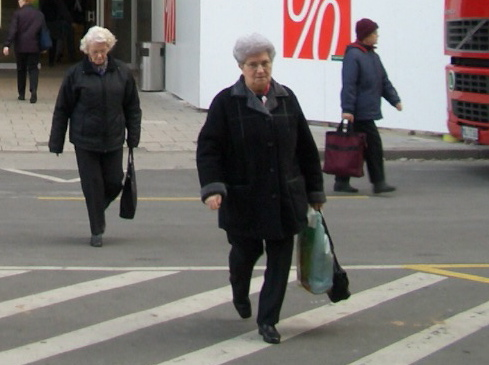
\includegraphics[width=0.5\linewidth]{img/vision/frame1.jpg}
	\caption{Pirâmide do conhecimento: modelo DIKW}
	\label{db}
\end{figure}


\textbf{Características: }
\begin{itemize}
	\item Dimensões (px): 
	\item Tamanho (MB): 
	\item Numero de pessoas existentes: 
\end{itemize}



\begin{longtable}{|l|l|l|l|l|l|} 
	\hline
	\textbf{winStride} & \textbf{padding} & \textbf{scale} & \textbf{detection (number)} & \textbf{execution time (seg)} \\ \hline
	(2, 2) & (8, 8) & 0.5 & 4 & 0.184819936752 \\ \hline
	(4, 4) & (8, 8) & 0.5 & 3 & 0.0488700866699 \\ \hline
	(8, 8) & (8, 8) & 0.5 & 1 & 0.0153889656067 \\ \hline
	(2, 2) & (8, 8) & 1.0 & 4 & 0.17699098587 \\ \hline
	(4, 4) & (8, 8) & 1.0 & 3 & 0.0484340190887 \\ \hline
	(8, 8) & (8, 8) & 1.0 & 1 & 0.0148591995239 \\ \hline
	(2, 2) & (8, 8) & 1.5 & 6 & 0.177606105804 \\ \hline
	(4, 4) & (8, 8) & 1.5 & 5 & 0.0484080314636 \\ \hline
	(8, 8) & (8, 8) & 1.5 & 2 & 0.0160319805145 \\ \hline
	(2, 2) & (16, 16) & 0.5 & 4 & 0.193215847015 \\ \hline
	(4, 4) & (16, 16) & 0.5 & 3 & 0.0518131256104 \\ \hline
	(8, 8) & (16, 16) & 0.5 & 1 & 0.0164451599121 \\ \hline
	(2, 2) & (16, 16) & 1.0 & 4 & 0.193369865417 \\ \hline
	(4, 4) & (16, 16) & 1.0 & 3 & 0.05233502388 \\ \hline
	(8, 8) & (16, 16) & 1.0 & 1 & 0.0161139965057 \\ \hline
	(2, 2) & (16, 16) & 1.5 & 6 & 0.193920850754 \\ \hline
	(4, 4) & (16, 16) & 1.5 & 5 & 0.0550818443298 \\ \hline
	(8, 8) & (16, 16) & 1.5 & 2 & 0.0162160396576 \\ \hline
	(2, 2) & (24, 24) & 0.5 & 4 & 0.203732967377 \\ \hline
	(4, 4) & (24, 24) & 0.5 & 3 & 0.0558068752289 \\ \hline
	(8, 8) & (24, 24) & 0.5 & 1 & 0.0173289775848 \\ \hline
	(2, 2) & (24, 24) & 1.0 & 4 & 0.203326940536 \\ \hline
	(4, 4) & (24, 24) & 1.0 & 3 & 0.0569319725037 \\ \hline
	(8, 8) & (24, 24) & 1.0 & 1 & 0.0179741382599 \\ \hline
	(2, 2) & (24, 24) & 1.5 & 6 & 0.20330619812 \\ \hline
	(4, 4) & (24, 24) & 1.5 & 5 & 0.0555651187897 \\ \hline
	(8, 8) & (24, 24) & 1.5 & 2 & 0.0173530578613 \\ \hline
	
		
	\caption{Your caption here} % needs to go inside longtable environment
	\label{tab:myfirstlongtable}
\end{longtable}


\newpage
\section{Frame 2}

\begin{figure}[h]
	\centering
	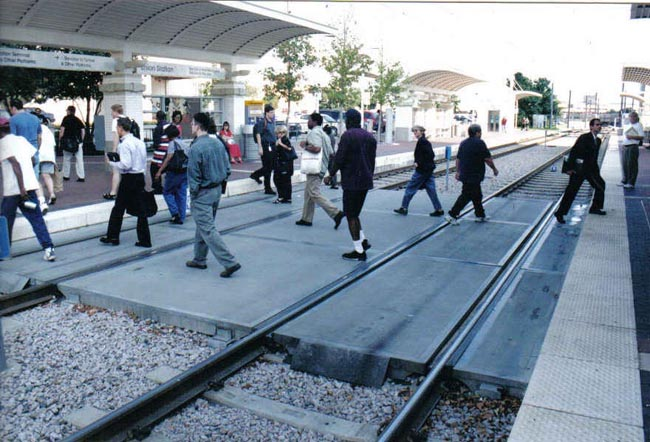
\includegraphics[width=0.5\linewidth]{img/vision/frame2.jpg}
	\caption{Pirâmide do conhecimento: modelo DIKW}
	\label{db}
\end{figure}


\begin{longtable}{|l|l|l|l|l|l|} 
	\hline
	\textbf{winStride} & \textbf{padding} & \textbf{scale} & \textbf{detection (number)} & \textbf{execution time (seg)} \\ \hline
	(2, 2) & (8, 8) & 0.5 & 11 & 0.335342168808 \\ \hline
	(4, 4) & (8, 8) & 0.5 & 4 & 0.0799450874329 \\ \hline
	(8, 8) & (8, 8) & 0.5 & 0 & 0.0238499641418 \\ \hline
	(2, 2) & (8, 8) & 1.0 & 11 & 0.293792009354 \\ \hline
	(4, 4) & (8, 8) & 1.0 & 4 & 0.0808959007263 \\ \hline
	(8, 8) & (8, 8) & 1.0 & 0 & 0.024552822113 \\ \hline
	(2, 2) & (8, 8) & 1.5 & 10 & 0.310877084732 \\ \hline
	(4, 4) & (8, 8) & 1.5 & 6 & 0.0828230381012 \\ \hline
	(8, 8) & (8, 8) & 1.5 & 1 & 0.031553030014 \\ \hline
	(2, 2) & (16, 16) & 0.5 & 11 & 0.356366157532 \\ \hline
	(4, 4) & (16, 16) & 0.5 & 5 & 0.0858371257782 \\ \hline
	(8, 8) & (16, 16) & 0.5 & 0 & 0.0261859893799 \\ \hline
	(2, 2) & (16, 16) & 1.0 & 11 & 0.324184179306 \\ \hline
	(4, 4) & (16, 16) & 1.0 & 5 & 0.0870020389557 \\ \hline
	(8, 8) & (16, 16) & 1.0 & 0 & 0.0258660316467 \\ \hline
	(2, 2) & (16, 16) & 1.5 & 10 & 0.321846008301 \\ \hline
	(4, 4) & (16, 16) & 1.5 & 7 & 0.0916659832001 \\ \hline
	(8, 8) & (16, 16) & 1.5 & 1 & 0.0345950126648 \\ \hline
	(2, 2) & (24, 24) & 0.5 & 11 & 0.343872070312 \\ \hline
	(4, 4) & (24, 24) & 0.5 & 5 & 0.0918598175049 \\ \hline
	(8, 8) & (24, 24) & 0.5 & 0 & 0.0270938873291 \\ \hline
	(2, 2) & (24, 24) & 1.0 & 11 & 0.344779968262 \\ \hline
	(4, 4) & (24, 24) & 1.0 & 5 & 0.090653181076 \\ \hline
	(8, 8) & (24, 24) & 1.0 & 0 & 0.0263440608978 \\ \hline
	(2, 2) & (24, 24) & 1.5 & 10 & 0.355221986771 \\ \hline
	(4, 4) & (24, 24) & 1.5 & 7 & 0.0967049598694 \\ \hline
	(8, 8) & (24, 24) & 1.5 & 1 & 0.0326068401337 \\ \hline


	\caption{Your caption here} % needs to go inside longtable environment
	\label{tab:myfirstlongtable}
\end{longtable}


\newpage
\section{Frame 3}


\begin{figure}[h]
	\centering
	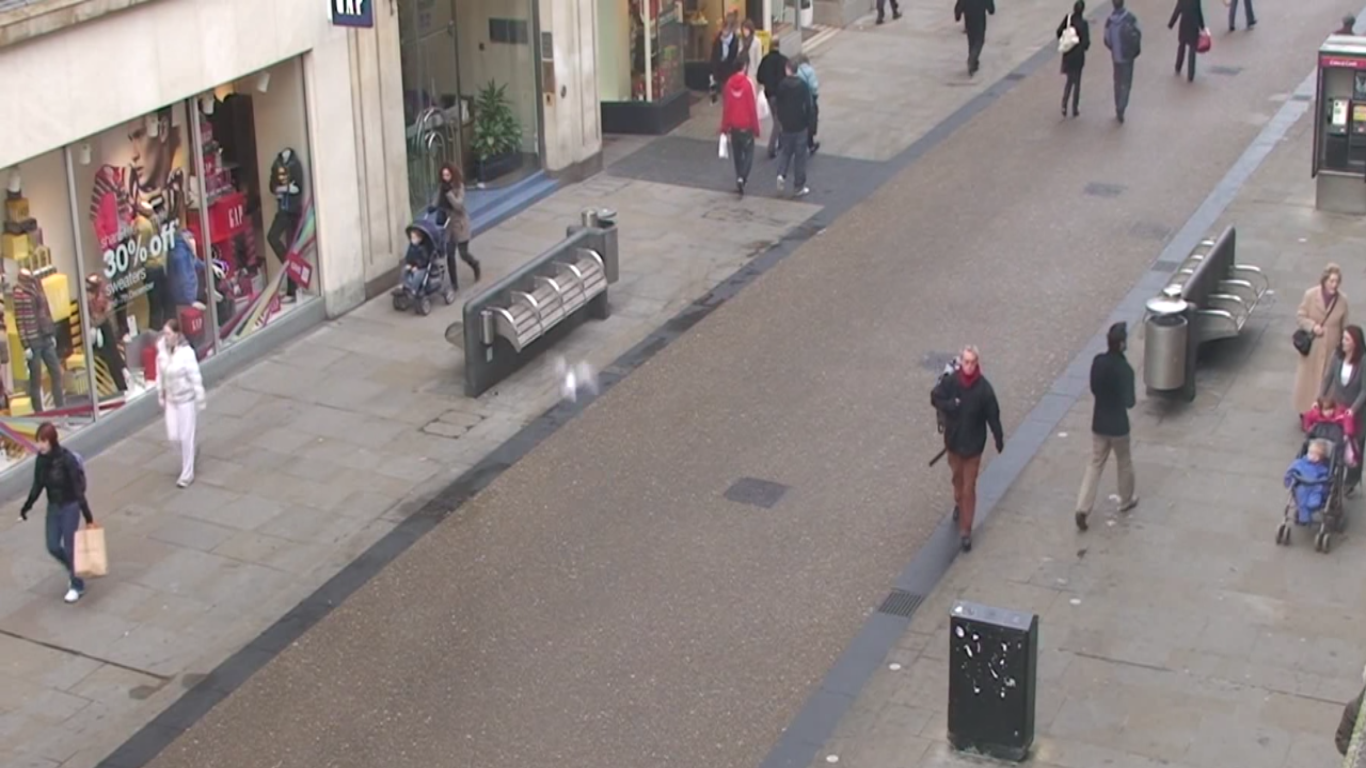
\includegraphics[width=0.5\linewidth]{img/vision/frame3.png}
	\caption{Pirâmide do conhecimento: modelo DIKW}
	\label{db}
\end{figure}




\begin{longtable}{|l|l|l|l|l|l|} 
	\hline
	\textbf{winStride} & \textbf{padding} & \textbf{scale} & \textbf{detection (number)} & \textbf{execution time (seg)} \\ \hline
	(2, 2) & (8, 8) & 0.5 & 8 & 1.25844407082 \\ \hline
	(4, 4) & (8, 8) & 0.5 & 5 & 0.359390974045 \\ \hline
	(8, 8) & (8, 8) & 0.5 & 1 & 0.131782054901 \\ \hline
	(2, 2) & (8, 8) & 1.0 & 8 & 1.27126002312 \\ \hline
	(4, 4) & (8, 8) & 1.0 & 5 & 0.355902910233 \\ \hline
	(8, 8) & (8, 8) & 1.0 & 1 & 0.131030082703 \\ \hline
	(2, 2) & (8, 8) & 1.5 & 16 & 1.26964783669 \\ \hline
	(4, 4) & (8, 8) & 1.5 & 12 & 0.364797115326 \\ \hline
	(8, 8) & (8, 8) & 1.5 & 1 & 0.197186946869 \\ \hline
	(2, 2) & (16, 16) & 0.5 & 8 & 1.3578350544 \\ \hline
	(4, 4) & (16, 16) & 0.5 & 5 & 0.357763051987 \\ \hline
	(8, 8) & (16, 16) & 0.5 & 1 & 0.132702112198 \\ \hline
	(2, 2) & (16, 16) & 1.0 & 8 & 1.27961397171 \\ \hline
	(4, 4) & (16, 16) & 1.0 & 5 & 0.367429971695 \\ \hline
	(8, 8) & (16, 16) & 1.0 & 1 & 0.132242918015 \\ \hline
	(2, 2) & (16, 16) & 1.5 & 17 & 1.28247308731 \\ \hline
	(4, 4) & (16, 16) & 1.5 & 12 & 0.403631925583 \\ \hline
	(8, 8) & (16, 16) & 1.5 & 1 & 0.207641839981 \\ \hline
	(2, 2) & (24, 24) & 0.5 & 8 & 1.43096494675 \\ \hline
	(4, 4) & (24, 24) & 0.5 & 5 & 0.369131088257 \\ \hline
	(8, 8) & (24, 24) & 0.5 & 1 & 0.134386062622 \\ \hline
	(2, 2) & (24, 24) & 1.0 & 8 & 1.34318900108 \\ \hline
	(4, 4) & (24, 24) & 1.0 & 5 & 0.371593952179 \\ \hline
	(8, 8) & (24, 24) & 1.0 & 1 & 0.134378194809 \\ \hline
	(2, 2) & (24, 24) & 1.5 & 17 & 1.39831089973 \\ \hline
	(4, 4) & (24, 24) & 1.5 & 13 & 0.444314002991 \\ \hline
	(8, 8) & (24, 24) & 1.5 & 1 & 0.137616872787 \\ \hline

	\caption{Your caption here} % needs to go inside longtable environment
	\label{tab:myfirstlongtable}
\end{longtable}






\newpage
\section{Frame 4}



\begin{figure}[h]
	\centering
	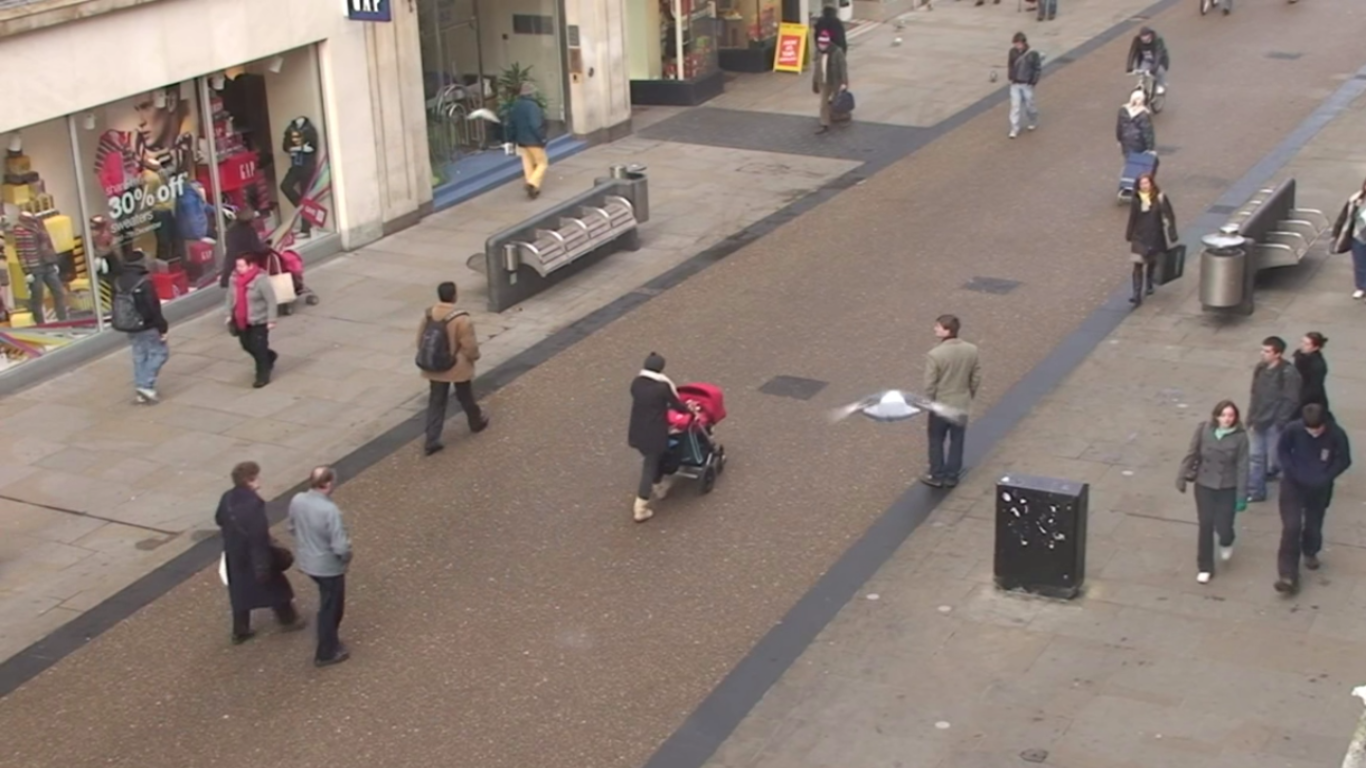
\includegraphics[width=0.5\linewidth]{img/vision/frame4.png}
	\caption{Pirâmide do conhecimento: modelo DIKW}
	\label{db}
\end{figure}


\begin{longtable}{|l|l|l|l|l|l|} 
	\hline
	\textbf{winStride} & \textbf{padding} & \textbf{scale} & \textbf{detection (number)} & \textbf{execution time (seg)} \\ \hline
	(2, 2) & (8, 8) & 0.5 & 7 & 1.3150138855 \\ \hline
	(4, 4) & (8, 8) & 0.5 & 2 & 0.36035490036 \\ \hline
	(8, 8) & (8, 8) & 0.5 & 0 & 0.129312992096 \\ \hline
	(2, 2) & (8, 8) & 1.0 & 7 & 1.24681711197 \\ \hline
	(4, 4) & (8, 8) & 1.0 & 2 & 0.358268976212 \\ \hline
	(8, 8) & (8, 8) & 1.0 & 0 & 0.130249023438 \\ \hline
	(2, 2) & (8, 8) & 1.5 & 17 & 1.58746790886 \\ \hline
	(4, 4) & (8, 8) & 1.5 & 12 & 0.513493061066 \\ \hline
	(8, 8) & (8, 8) & 1.5 & 1 & 0.197572946548 \\ \hline
	(2, 2) & (16, 16) & 0.5 & 7 & 1.36501693726 \\ \hline
	(4, 4) & (16, 16) & 0.5 & 2 & 0.363034009933 \\ \hline
	(8, 8) & (16, 16) & 0.5 & 0 & 0.132270812988 \\ \hline
	(2, 2) & (16, 16) & 1.0 & 7 & 1.29145503044 \\ \hline
	(4, 4) & (16, 16) & 1.0 & 2 & 0.359399080276 \\ \hline
	(8, 8) & (16, 16) & 1.0 & 0 & 0.132076025009 \\ \hline
	(2, 2) & (16, 16) & 1.5 & 19 & 1.61724209785 \\ \hline
	(4, 4) & (16, 16) & 1.5 & 13 & 0.467741012573 \\ \hline
	(8, 8) & (16, 16) & 1.5 & 1 & 0.170053005219 \\ \hline
	(2, 2) & (24, 24) & 0.5 & 7 & 1.33659911156 \\ \hline
	(4, 4) & (24, 24) & 0.5 & 2 & 0.365787982941 \\ \hline
	(8, 8) & (24, 24) & 0.5 & 0 & 0.133852005005 \\ \hline
	(2, 2) & (24, 24) & 1.0 & 7 & 1.29908204079 \\ \hline
	(4, 4) & (24, 24) & 1.0 & 2 & 0.377649784088 \\ \hline
	(8, 8) & (24, 24) & 1.0 & 0 & 0.13329410553 \\ \hline
	(2, 2) & (24, 24) & 1.5 & 19 & 1.32506895065 \\ \hline
	(4, 4) & (24, 24) & 1.5 & 13 & 0.38186788559 \\ \hline
	(8, 8) & (24, 24) & 1.5 & 1 & 0.1673848629 \\ \hline
	
	
	\caption{Your caption here} % needs to go inside longtable environment
	\label{tab:myfirstlongtable}
\end{longtable}











